\chapter{Probability}

% take from 132: 2-D prob mass ftn, marble ex, as generaliz of 1-D;
% covarince as extensive of variance in 1-D; correl is scaled version;
% define in terms of rho, sigmas; MovieLens ex!!!!; age, userMean,
% Nuser; rho in [-1,1] by Cauchy-Schwartz (optional)

It is assumed the reader has background in calculus-based probability
constructs, e.g.\ density functions and distributions involving
infinite series.  Here we treat some advanced topics used in the sequel.

\section{Multivariate Distributions}

\subsection{Multivariate Probability Mass Functions}
\label{marblepmf} 

Recall that for a single discrete random variable $X$, the distribution of
$X$ is defined to be a list of all the values of $X$, together with the
probabilities of those values.  We encapsulate those in the
\textit{probability mass function}:

\begin{equation}
p_X(i) = P(X = i)
\end{equation}

Here the argument is $i$.

So, if $X$ is the number of heads in two flips of a coin, $p_X(0) =
1/4$, $p_X(1) = 1/2$ and $p_X(2) = 1/4$. 

This is extended to a pair of discrete random variables $U$ and $V$ as

\begin{equation}
p_{U,V}(i,j) = P(U = i, V = j)
\end{equation}

with arguments $i$ and $j$.

For example, suppose we have a bag containing two yellow marbles, three
blue ones and four green ones.  We choose four marbles from the bag at
random, without replacement.  Let $Y$ and $B$ denote the number of yellow
and blue marbles that we get.  Then

\begin{equation}
p_{Y,B}(i,j) = P(Y = i \textrm{ and } B = j) = 
\frac
{
\binom{2}{i}
\binom{3}{j}
\binom{4}{4-i-j}
}
{\binom{9}{4}}
\end{equation}

Here is a table displaying all the values of $p_{Y,B}(i,j)$

\begin{tabular}{|r|r|r|r|r|r|}
\hline
i $\downarrow$, j $\rightarrow$ & 0 & 1 & 2 & 3 \\ \hline
0 & 0.0079 & 0.0952 & 0.1429 & 0.0317 \\ \hline
1 & 0.0635 & 0.2857 & 0.1905 & 0.1587 \\ \hline
2 & 0.0476 & 0.0952 & 0.0238 & 0.000 \\ \hline
\end{tabular}

So in our marble example above, $p_{Y,B}(1,2) = 0.048$, $p_{Y,B}(2,0) =
0.012$ and so on.

\subsection{Multivariate Density Functions}

Recall that for a continuous random variable $X$, we can find
probabilities involving $X$ by integrating its density:

\begin{equation}
P(X \textrm{ in } A) = \int_{A} f_X(t) ~ dt
\end{equation}

for regions $A$ in the real line.

This extends to multiple dimensions.  For sets $A$ in the plane,

\begin{equation}
P[(X,Y) \textrm{ in } A] = \int_{A} \int f_{X,Y}(s,t) ~ ds  ~ dt
\end{equation}

The density for $k$ random variables $X_1,...,X_k$ is likewise a
function whose $k$-fold integrals are probabilities.  

We almost never compute such integrals.  Instead, we rely on
approximations, including simulation.  The R package \textbf{mvtnorm}
can be used for these purposes.

\section{Relations Between Variables}

\subsection{Covariance}

You have seen the \textit{variance} of a single random variable before,

\begin{equation}
Var(X) = E[(X - EX)^2]
\end{equation}

It is a measure of \textit{dispersion}, i.e.\ how much $X$
varies in repeated realizations.\footnote{If we look at many instances
of a random variable $X$, they are called \textit{realizations}.}

In the example above in which $X$ is the number of heads obtained in two
flips of a coin, one can show that $EX = 1$ and
$Var(X) = 2(0.5)(1-0.5) = 0.5$.  So, if we look at many, many
realizations of $X$, the long-run average value of $X$ will be 1,
and the long-run average of $(X - 1)^2$ will be 1/2.

The \textit{standard deviation} of $X$, denoted here by $\sigma(X)$,
is defned at $\sqrt{Var(X)}$.  Recall that for a constant, i.e.\ a
nonrandom quantity, $c$, we have

\begin{equation}
\sigma(cX) = c \sigma(X)
\end{equation}

and 

\begin{equation}
\sigma(X+c) = \sigma(X)
\end{equation}

The reader should make sure both of these make intuitive sense.  For
instance, in the second case, the reasoning is:  Set $Y = X + c$.  In
repeated realizations, $Y$ will vary from its mean exactly as $X$
varies from its mean.

How does this extend?  The answer is the \textit{covariance}:

\begin{equation}
Cov(X,Y) = E[(X - EX) (Y - EY)]
\end{equation}

Just as $Var(X)$ is a measure of how much $X$ varies, the covariance is
a measure of how $X$ and $Y$ vary \textit{together}.  Note that it is a
signed quantity.

Think of height and weight in a human population, $X$ and $Y$. People
who are taller than average tend to be heavier than average, making

\begin{equation}
(X - EX) (Y - EY) > 0
\end{equation}

Shorter people tend to be lighter than average, but again

\begin{equation}
(X - EX) (Y - EY) > 0
\end{equation}

Now, 

\begin{equation}
E[(X - EX) (Y - EY)]
\end{equation}

is the average value of that product, as we range through various people
in the population, so the covariance will be positive.  
$(X - EX) (Y - EY)$ won't be positive for all people, but if the
relation is typical enough, the average will be positive.

Note that $Cov(X,X) = Var(X)$.

\subsection{Covariance Matrices}

Say we have $p$ random variables $X_1$,..., $X_p$.  Their
\textit{covariance matrix} is $p \times p$, with the $(i,j)$
element being $Cov(X_i,X_j)$.  The diagonal elements are the variances
of the individual variables.

\section{Correlation}

Roughly speaking, positively-related variable will have
positive covariance, with a similar statement for negatively-related
variables.  In fact, correlation is just scaled-down variance:

\begin{equation}
\rho(X,Y) = 
\frac{Cov(X,Y)}{\sigma(X) ~ \sigma(Y)}
\end{equation}

where $\rho$ and $\sigma$ are standard symbols for correlation and
standard deviation, respectively.

Correlation is unitless.  E.g.\ if $X$ and $Y$ are measured in meters,
the meter units cancel.  One can show that 

\begin{equation}
\label{rho11}
-1 \leq \rho \leq 1
\end{equation}

\subsection{Proof of (\ref{rho11}) by Vector Spaces}

Let $\mathcal{W}$ be the set of all random variables with mean 0 and
finite
variance (in some setting).  We lose no generality in assume mean 0,
since replacing a random variable $U$ by $U - EU$ makes the mean 0 and
does not change the correlation.

$\mathcal{W}$is clearly closed under linear combinations, and we can
define an inner product (``dot product'') by

\begin{equation}
<U,V> = Cov(U,V)
\end{equation}

The vector norm will be

\begin{equation}
||U|| = (<U,U>)^{0.5} = \sigma(U)
\end{equation}

To qualify as an inner product, it must be symmetric and linear in both
arguments, and must be \textit{positive definite}, i.e. $<U,U> \geq 0$,
with equality if and only if $U = 0$.  Covariance satisfies all these
conditions. 

On any inner product space, the Cauchy-Schwarz Inequality says that the
absolute value of the inner product of two vectors, divided by the
product of their norms, is at most 1.  That gives us (\ref{rho11})!

So, is a correlation of, say, 0.4, large or small?  It is customary to
gauge this by the squared correlation, which arises in the theory of
linear predictors (Chapter \ref{chap:ml}).  The quantity $\rho^2$ can be
shown to be the reduction in mean squared prediction error when we
predict $V$ using $U$ (or vice versa).

\subsection{Is a Correlation Large or Small?}

Say we want to predict $V$ knowing $U$.  Intutively, the larger
$\rho(U,V)$ is, the more accurately I can predict.  This can be quantified.

Let's consider predictors of the form

\begin{equation}
\label{predv}
\widehat{V} = c_1 + c_2 U
\end{equation}

$\widehat{V}$ means the predicted value of $V$

There are optimal choices for the $c_i$, but let's not get into that for
now.

Our \textit{mean squared prediction error} is then

\begin{equation}
\textrm{MSPE}_1 = E[(V - \widehat{V})^2]
\end{equation}

But what if we don't know $U$?  Then we can't use (\ref{predv}).  In
that case, a reasonable guess for $V$ would be $EV$.  Then our MSPE
would be

\begin{equation}
\textrm{MSPE}_2 = E[(V - EV)^2]
\end{equation}

You'll recognize the latter as $Var(V)$, but the main point here is that
it turns out that

\begin{equation}
\rho^2(U,V) =
\frac{MSPE_2 - MSPE_1}{MSPE_2}
\end{equation}

In other words, the squared correlation can be interpreted as the
proportional reduction in MSPE that we attain by using $U$ to predict
$V$ instead of using $EV$ to do so.  This is often described as ``The
proportion of variation in $V$ that is explainable by $U$.''

\subsection{Example:  MovieLens}

Again, \textbf{ml100kpluscovs} is MovieLens plus some side information:

\begin{lstlisting}
 head(ml100kpluscovs)
  user item rating timestamp age gender        occ   zip userMean Nuser G1 G2
1    1    1      5 874965758  24      M technician 85711 3.610294   272  0  0
2  117    1      4 880126083  20      M    student 16125 3.918605    86  0  0
3  429    1      3 882385785  27      M    student 29205 3.393720   414  0  0
4  919    1      4 875289321  25      M      other 14216 3.470046   217  0  0
5  457    1      4 882393244  33      F   salesman 30011 4.025271   277  0  0
6  468    1      5 875280395  28      M   engineer 02341 3.993007   143  0  0
  G3 G4 G5 G6 G7 G8 G9 G10 G11 G12 G13 G14 G15 G16 G17 G18 G19 itemMean Nitem
1  0  1  1  1  0  0  0   0   0   0   0   0   0   0   0   0   0 3.878319   452
2  0  1  1  1  0  0  0   0   0   0   0   0   0   0   0   0   0 3.878319   452
3  0  1  1  1  0  0  0   0   0   0   0   0   0   0   0   0   0 3.878319   452
4  0  1  1  1  0  0  0   0   0   0   0   0   0   0   0   0   0 3.878319   452
5  0  1  1  1  0  0  0   0   0   0   0   0   0   0   0   0   0 3.878319   452
6  0  1  1  1  0  0  0   0   0   0   0   0   0   0   0   0   0 3.878319   452
\end{lstlisting}

(The G's are genres.)

Let's find some correlations:\footnote{These are only \textit{sample}
correlations.  Our data are regarded as a sample from a \textit{population}
of data from all possible users and all possible movies.}

\begin{lstlisting}
> cor(ml100kpluscovs[,c('age','userMean','Nuser')])
                 age   userMean       Nuser
age       1.00000000  0.1355457 -0.03908845
userMean  0.13554566  1.0000000 -0.30755257
Nuser    -0.03908845 -0.3075526  1.00000000
\end{lstlisting}

There seems to be rather little relation betwen age and the mean rating
for a user, and between age and the number of ratings for a user.  But
the latter two variables seem to have a negative relation---still rather
weak, with each variable explaining about 9\% of the variation of the
other; users who give higher ratings rate fewer movies.

We might ask, say, whether any genres are related to each other:

\begin{lstlisting}
# some rows are all NAs
> cc <- complete.cases(ml100kpluscovs[,11:29]) 
> w <- ml100kpluscovs[cc,]
> cor(w[,11:19])
            G11          G12          G13          G14          G15         G16
G11  1.00000000 -0.031493550 -0.030273614  0.232039913 -0.055267116  0.01614678
G12 -0.03149355  1.000000000 -0.054022202  0.001783286 -0.076165496  0.03418726
G13 -0.03027361 -0.054022202  1.000000000 -0.053634780 -0.009765185 -0.08138982
G14  0.23203991  0.001783286 -0.053634780  1.000000000 -0.059997502 -0.03084474
G15 -0.05526712 -0.076165496 -0.009765185 -0.059997502  1.000000000 -0.06345353
G16  0.01614678  0.034187257 -0.081389822 -0.030844736 -0.063453529  1.00000000
G17  0.11025056  0.069788805 -0.111244337  0.230288448 -0.106256128  0.04679552
G18 -0.04280364 -0.076381585 -0.055381372 -0.075833813  0.126545414  0.16727458
G19 -0.01826573 -0.032594547 -0.031331963 -0.032360794 -0.052448355 -0.05253437
            G17         G18         G19
G11  0.11025056 -0.04280364 -0.01826573
G12  0.06978881 -0.07638159 -0.03259455
G13 -0.11124434 -0.05538137 -0.03133196
G14  0.23028845 -0.07583381 -0.03236079
G15 -0.10625613  0.12654541 -0.05244835
G16  0.04679552  0.16727458 -0.05253437
G17  1.00000000 -0.10041124 -0.07278201
G18 -0.10041124  1.00000000 -0.02372091
G19 -0.07278201 -0.02372091  1.00000000
\end{lstlisting}

There may be some slight relations.

\subsection{An Important Matrix Property}

Say we have a random \textit{vector} $X$, length $p$, and a $k \times p$
nonrandom matrix $A$.  Then $AX$ is a new random vector, of length $k$.
One can show that

\begin{equation}
Cov(AX) = A ~ Cov(X) ~ A'
\end{equation}

where here $Cov()$ with a single argument means covariance matrix, and
$'$ denotes transpose.

An important special case is that in which $A$ is a row vector.  Then
$AX$ is a number, and $Cov(AX)$ reduces to $Var(AX)$.

\section{The Normal (Gaussian) Family of Distributions}

\subsection{Univariate}

The density function here is the famous ``bell-shaped curve,''

\begin{equation}
f_X(t) = \frac{1}{\sqrt{2\pi} c}
\exp
{
\left ( -0.5 \left [ (t-b)/c  \right ]^2 
\right )
}
\end{equation}

This is a parametric family of curves.  Here $b$ and $c$ are parameters.
They also turn out to be the mean and standard deviation of the
distribution.  Notation for this distribution is $\textrm{N}(a,b^2)$.

This is a very common model, as a histogram of one's data often looks
rather bell-shaped.  Here is one from MovieLens:

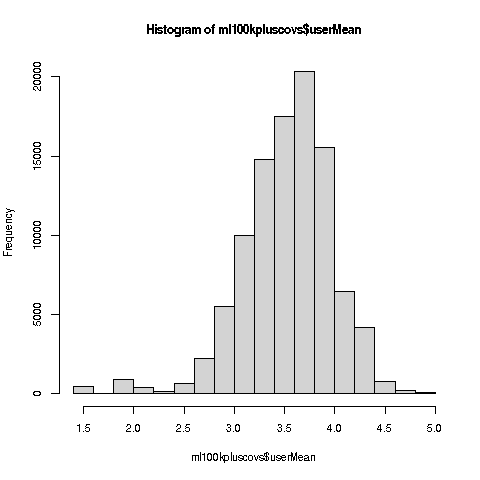
\includegraphics[width=3.6in]{Images/HistUserMean.png} 

There are lots of issues here, e.g.\ ``How close must the histogram
be to bell-shaped in order for us to use it as a model?''  More on this
in Chapter \ref{chap:stat}.

One reason that random variables in practice tend to be approximately
normal is the \textit{Central Limit Theorem}, which says that if a
random variable $X$ is a sum of many random variables, then its
distribution is approximately normal even if the individual terms are
not normal.  An example is human height.  Think of the body as made up
of a number of chunks.  The person's height is the sum of the heights of
the chunks.  This is a rough analysis, actually based on advanced
versions of the theorem, but in fact human height \textit{is}
approximately normally distributed.  (Try running a histogram on the
height column in the \lstinline{mlb} dataset that comes with
\lstinline{regtools}.)

\subsection{Multivariate}

If we have two random variables $X$ and $Y$, they have a
\textit{bivariate normal distribution} if their density looks like a
``three-dimensional bell.''  We will skip the exact density (for $p$
variables).

Below are graphs of example bivariate normal densities, one with $\rho =
0.2$ and the other with $\rho = 0.8$.

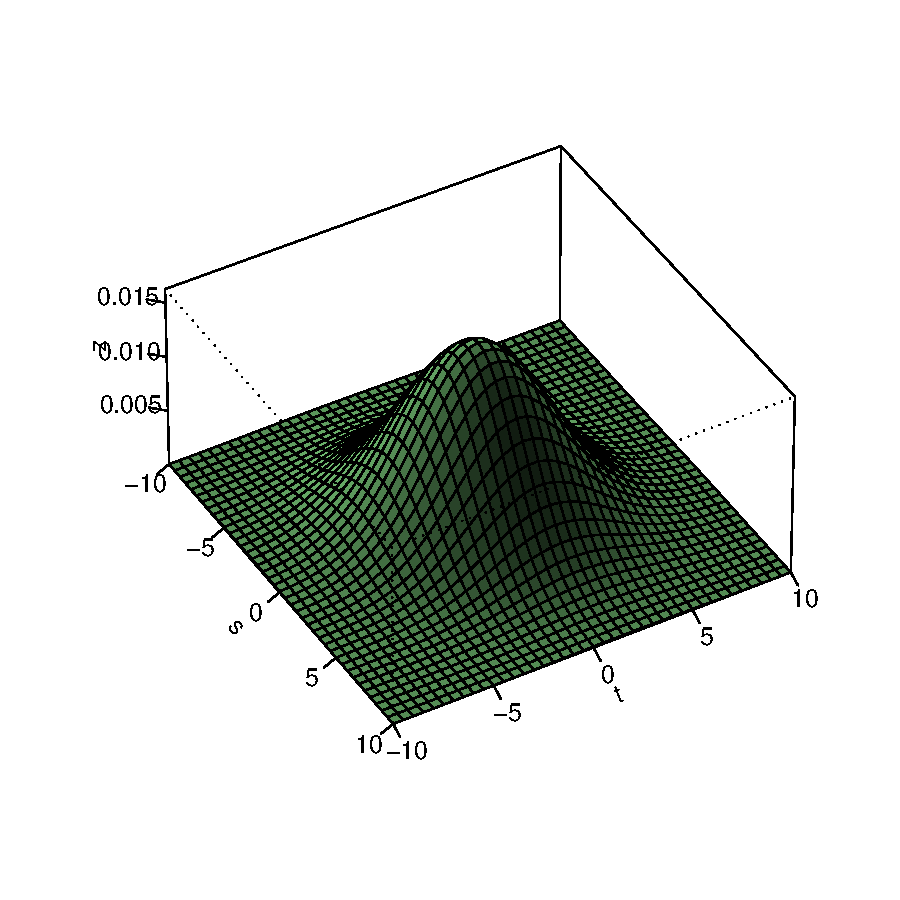
\includegraphics[width=3.6in]{Images/Rho2.pdf} 
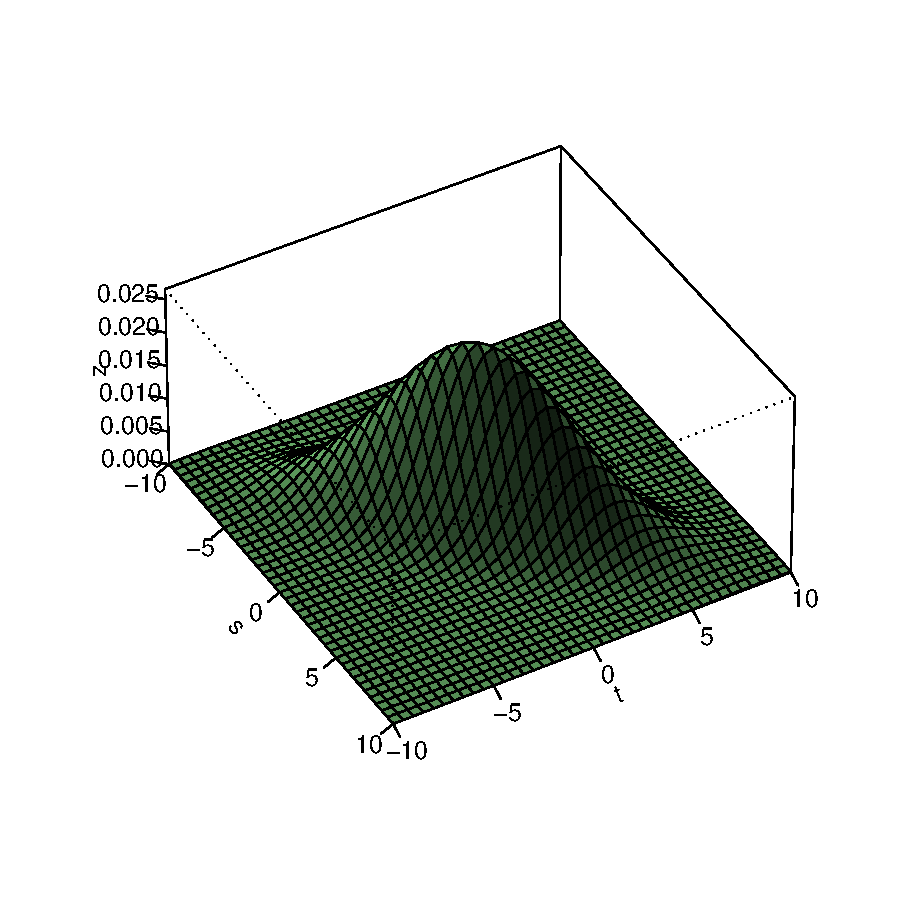
\includegraphics[width=3.6in]{Images/Rho8.pdf} 

You can see the effect of a higher correlation in the second graph; the
bell is hugging a line at the base, so the two variables tend to be
large together or small together.

\section{Mixture Distributions}

\subsection{Motivating Example}

The \lstinline{faithful} dataset included in R consists of data from the
Old Faithful geyser in Yellowstone National Park, USA.  Let's take a
look at times between eruptions:

\begin{lstlisting}
> plot(density(faithful$waiting)) 
\end{lstlisting}

Here we are using a more sophisticated density estimator than
\lstinline{hist()}, \lstinline{density()}.  It gives smooth curves.

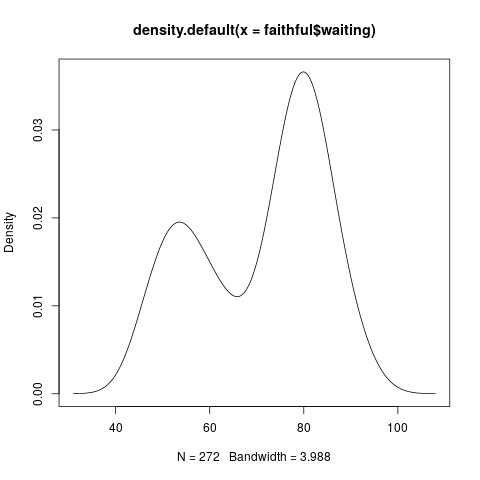
\includegraphics[width=3.6in]{Images/DensFaithful.png} 

We might say it's a ``double bell.''  What's at work here?

It looks like a \textit{mixture} of two normals, meaning that possibly
two underground mechanisms are causing eruptions, sometimes mechanism A
and sometimes mechanism B.  If the wait times between events is normal
for each mechanism, we would get the ``double bell'' appearance.

To understand this better, consider this simulation experiment:

\begin{lstlisting}
> x1 <- rnorm(2500) 
> x2 <- rnorm(2500)+5 
> i <- sample(c(TRUE,FALSE),1000,replace=TRUE) 
> x <- ifelse(i,x1,x2) 
> plot(density(x))
\end{lstlisting}

Here we generated 2500 random values each from 
$\textrm{N}(0,1)$ and $\textrm{N}(5,1)$, but formed \lstinline{x}
by randomly choosing from those two sets of 2500.  (We slightly favored
the second one.)

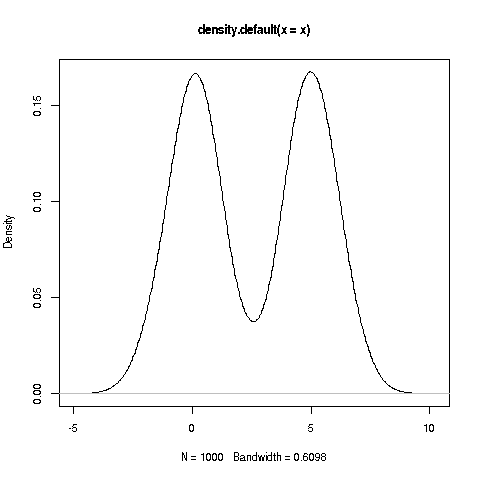
\includegraphics[width=3.6in]{Images/MixSim.png} 

Sure enough, we got a double bell.

One can use a technique known as the \textit{EM algorithm} to estimate
the parameters of the two normals, plus the proportion of each.  The R
package \lstinline{mixtools} does the computation.

\subsection{Clustering Algorithms and Use in RS}

\textit{Clustering} methods are exploratory tools to find mixtures.  In
the Old Faithful example, it was rather clear that there was a mixture
of two normals, but in general it's much, much harder, for a couple of
reasons:

\begin{itemize}

\item We are usually in a multivariate setting, rather than the
univariate one in the Old Faithful example.

\item The number of mixing components, 2 in the above example, is not
clear at all.

\end{itemize} 

Various methods have been devised, and have been found useful in RS,
such as in \textit{market segmentation}.  We may find that moviegoers,
for instance, tend to fall into, say, 5 main groups.  We will return to
this later.
